This mode is proposal in the classic Kloeden's Book. \\ 
Peter Kloeden \& Eckhard Platen. Numerical Solution of Stochastic Differential Equations.
$$
	\ddot{x}+\dot{x}-(\alpha-x^2)x=\sigma \varepsilon
$$
\begin{align}
	dX_t^{(1)}&= X_t^{(2)} dt \label{eqn:SimDuffingVanDerPolSDE1}\\
	dX_t^{(2)}&=
		\left\{
		X_t^{(1)}
		\left(
			\alpha-(X_t^{(1)})^2
		\right)
		-X_t^{(2)}
	\right\}dt
	+\sigma X_t^{(1)} dW_t \label{eqn:SimDuffingVanDerPolSDE2}
\end{align}
The Steklov Scheme:
\begin{align}
	X^{(1)}_{k+1} &= X^{(1)}_{k} + h X^{(2)}_{k} \notag \\
	X^{(2)}_{k+1} & = a\left(X^{(1)}_{k},X^{(1)}_{k+1}\right)
		\left(
			1 - \exp(-h)
		\right)
		+ \exp(-h) X^{(2)}_{k} + \sigma X^{(1)}_{k} \Delta W_k. \label{eqn:SteklovSimDuffingVanDerPol}\\
		a\left(x, y\right) & = x (\alpha - xy) \notag
\end{align}
In this way also we has been constructed a SSLS for SDE 
\crefrange{eqn:SimDuffingVanDerPolSDE1}{eqn:SimDuffingVanDerPolSDE2} given by
\begin{align}
	X_{k+1}^{(1)} & = X_{k}^{(1)} + h X_{k}^{(2)} \notag\\
	X_{k+1}^{(2)} & = X_{k}^{(2)} 
		\left(
			\exp(-h) - a_2^{(2)}\left(X_{k+1}^{(1)}\right)
		\right) + a_2^{(2)}\left(X_{k+1}^{(1)}\right) 
		+ \sigma X_{k}^{(1)} \Delta W_k
		\label{eqn:SimDuffingVanDerPolSSLS2}\\
		a_2^{(2)}(x) & = x (\alpha - x^2) \notag
\end{align}
In \Cref{fig:SimplifyedDuffingVanDerPolSDE} we present a likening between the EM, two Steklov methods and the Balanced
Implicit scheme (see e.g \cite{Alcock2006}).
\newgeometry{left=1.75cm, bottom=3cm}
\begin{figure}[h!]
	\centering
	\subfloat[]{
		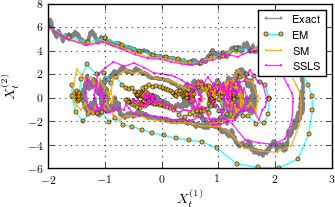
\includegraphics{./papers/paperB/figures/PhasePotraitSimDuffingVanDerPol}
		\label{fig:PhasePotraitSimDuffingVanDerPol}
	}\\
	\subfloat[]{
		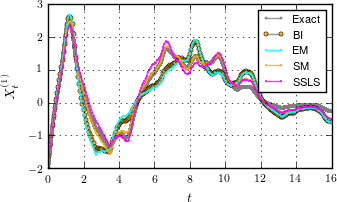
\includegraphics{./papers/paperB/figures/X1SimDuffingVanDerPol.png}
		\label{subfig:X1SimplifiedVanDerPol}
	}
		\subfloat[]{
			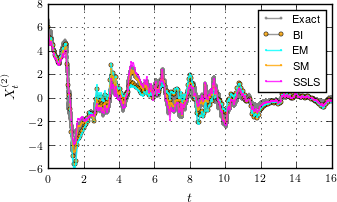
\includegraphics{./papers/paperB/figures/X2SimDuffingVanDerPol.png}
			\label{subfig:X2SimplifiedVanDerPol}
		}
	\caption{Numerical sample paths of SDE \crefrange{eqn:SimDuffingVanDerPolSDE1}{eqn:SimDuffingVanDerPolSDE2}
		with the Euler-Maruyama (EM), Steklov-Mickens (SM) Balanced Implicit(BI) and SSLS methods.
		We set the parameters of the underlying SDE with 
		$\alpha = 1$, 
		$\sigma = 2$,
		$X_0 = (-2, 6)$,
		and fixed the stencil simulation at $h = 2^{-4}$ over the time interval $[0,16]$.
	}
	\label{fig:SimplifyedDuffingVanDerPolSDE}
\end{figure}
\restoregeometry
Gives good results.

